\section{Simulation Setup}

\section{Simulations}

The dispatching algorithms as presented before have been tested in the agent-
and activity-based transport simulation framework MATSim. What has been used in
this paper is the mobility simulation component of that package, where each agent
has a daily plan consisting of activities and legs. Activities are performed for a
certain duration at specific locations in the traffic network and have predefined
end times. They are connected by legs, which are performed by specific means of
transport. Dependent on the time of day, the mode, the route taken and other factors,
travel times may vary. Most importantly, the network is capacitated such that
congestion emerges if many agents use the same networks links at the same time.

Most important for the study at hand is the simulation of vehicles in an actual
network. By keeping background traffic in the simulation, the AVs are constrained
by the network conditions, most remarkably they suffer from longer travel times
at peak hours due to congestion.

The section is divided into two parts: First, we describe how the simulation
scenario has been set up to account for a realistic travel demand for Zurich.
Second, the simulation approach for automated vehicles is explained and third,
the results for the different dispatching algorithms are presented.

\begin{figure}[h]
\begin{center}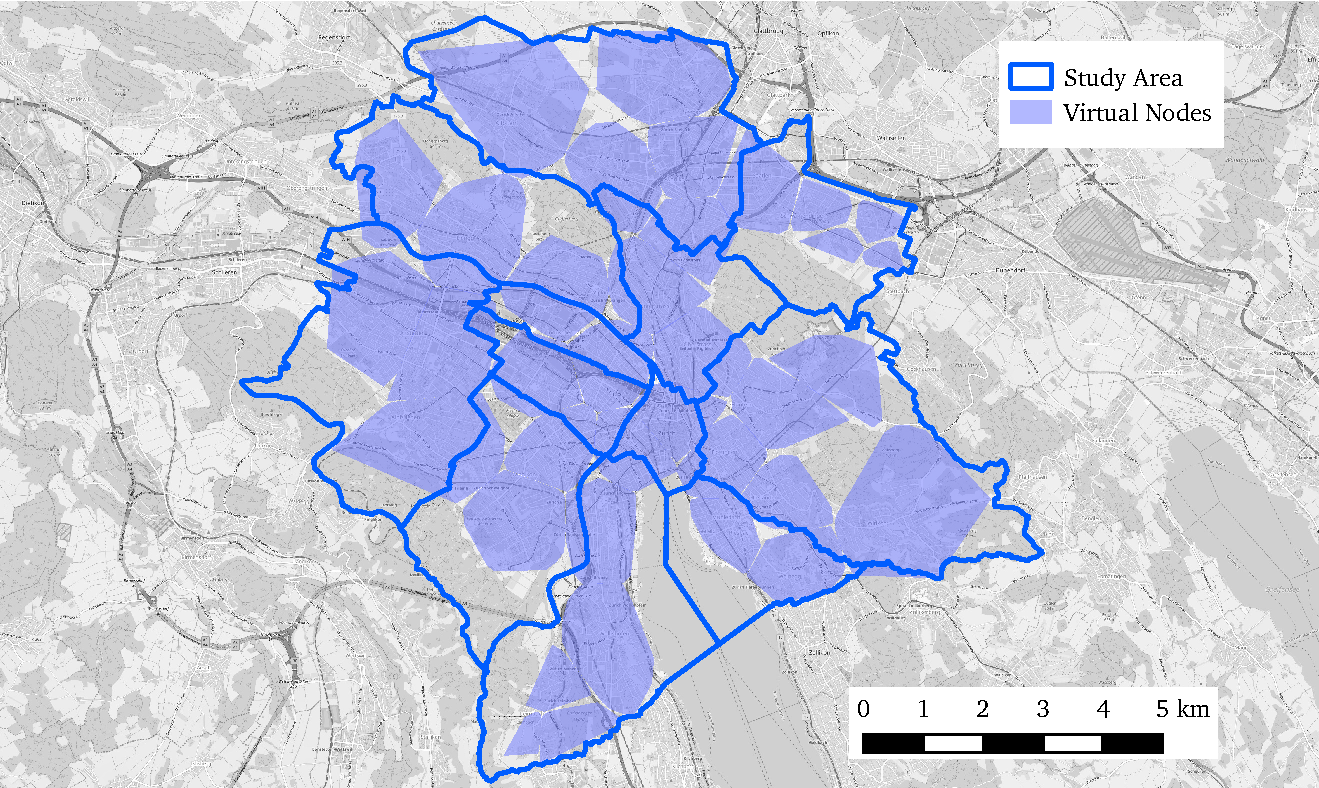
\includegraphics[width=1.0\textwidth]{figures/map.pdf}\end{center}
\caption{The study area covering the 12 districts of Zurich and the nodes of the virtual network for the rebalancing algorithms.}
\label{fig:study_area_vnodes}
\end{figure}
